\documentclass[11pt]{report}
\usepackage[utf8]{inputenc}
\usepackage[T1]{fontenc}
\usepackage{amsmath,amssymb,amsfonts}
\usepackage{booktabs}
\usepackage{geometry}
\geometry{letterpaper,margin=1in}
\usepackage{microtype}
\usepackage[table]{xcolor}
\usepackage{tikz}
\usetikzlibrary{shapes,arrows,positioning,calc,decorations.pathmorphing,backgrounds}
\usepackage{float}
\usepackage{mdframed}
\usepackage{hyperref}
\hypersetup{
    colorlinks=true,
    linkcolor=teal,
    citecolor=teal,
    urlcolor=teal
}

\newmdenv[
  linecolor=black,
  linewidth=1pt,
  innertopmargin=10pt,
  innerbottommargin=10pt,
  innerrightmargin=12pt,
  innerleftmargin=12pt,
  backgroundcolor=gray!5
]{blackboard}

\title{\Huge\textbf{The Feynman Lectures on Courtship Mechanics}\\
\Large The Classical Dynamics of Friendship, Commitment, and Holy Covenant}
\author{\textbf{Adam Matthew Steinberger}}
\date{November 2026}

\begin{document}

\maketitle

\tableofcontents
\newpage

\chapter*{Preface}
\addcontentsline{toc}{chapter}{Preface}

Most people believe romantic love is a mystical fog where rational thought ceases to function. They assume feelings will guide them to happiness, ignoring the laws of human nature.

In physics, if an engineer builds a suspension bridge based on wishes, ignoring gravity, tension, and metallurgical stress limits, the cables snap and the bridge plunges into the gorge. Human relationships obey equally unyielding laws. When people ignore human fallenness, such as the reality that spouses lie, break trust, conceal motives, and betray vows, catastrophic relational collapse follows.

The first principle is that you must not fool yourself, and you are the easiest person to fool. In these lectures, we examine the mechanics of Christian courtship: the transition from community friendship to solemn engagement and indissoluble covenant marriage. We study the two springs of commitment formulated by Scott Stanley, the thermal regulation of Murray Bowen's differentiation of self, the three historical pillars of Protestant covenant, Catholic sacramental depth, and Greek Orthodox ascetical crowns, and the non-negotiable physical guardrail of premarital chastity.

\chapter{The Principle of Least Action and the Nature of Covenants}

\section{The Office Hours After the Heartbreak}
The door to 103 Bridge Annex stood open. Chalk dust hung in the afternoon sunlight. On the center slate, between Maxwell equations, Professor Richard Feynman had chalked a bold question: \textit{``What is the binding energy of a human promise?''}

Daniel walked into the office, his notebook tucked under his arm. He looked exhausted.

``Come in, Daniel!'' Feynman said, spinning a wooden gyroscope on his desk. ``Sit down before you fall over. You look like you tried to push a locomotive up a grease-covered hill. What went wrong?''

``Everything, Professor,'' Daniel said, sitting heavily on the wooden chair. ``My personal life feels like a pile of scrap iron. You know my history: married young, thought love was pure emotion. We slid into marriage with zero sober evaluation. When the machine shop hit financial trouble and my daughter Maddie needed round-the-clock care, my former wife checked out. She abandoned us. It turned out she never shared my faith. Paul speaks of this in First Corinthians seven, fifteen: the departure of an unbelieving spouse. The divorce nearly crushed me. I know marriage is meant to be a permanent, once-in-a-lifetime union. Living through that failure felt like dying. Now my friendship with Nora has deepened, and we are talking about courtship. I am terrified of repeating past wreckage.''

Feynman stopped the gyroscope with his finger. ``Good. Terror is the beginning of engineering wisdom. An engineer who survived a bridge collapse respects load limits.''

``How do we analyze courtship scientifically?'' Daniel asked.

``Start with the difference between a contract and a covenant,'' Feynman said, grabbing a piece of chalk. ``In classical mechanics, a particle moves along a path that minimizes the action. In human society, a contract is a transactional game with finite stopping times. Two parties cooperate while the short-term payoff exceeds alternative options:
\begin{equation}
U_{\text{contract}} = \sum_{t=0}^{T} \delta^t \Big( \pi_i(a_{i,t}, a_{j,t}) - c_i(a_{i,t}) \Big)
\end{equation}
If your business partner or your spouse suffers an economic panic, gets sick, or becomes difficult, the contract incentive drops below zero. The selfish player defects. That is what happened in your first marriage: an unexamined contract masquerading as love.''

``What is a covenant?'' Daniel asked.

``A covenant is an infinite-potential well,'' Feynman said, striking the board with chalk. ``In quantum mechanics, when an electron falls into an infinitely deep potential well, it requires infinite energy to escape. It is permanently bound. Christian marriage is an indissoluble covenant before Almighty God. It is an irreversible transformation:
\begin{equation}
U_{\text{covenant}} = \mathbb{E} \left[ \sum_{t=0}^{\infty} \beta^t \Big( W(s_t) + \lambda \cdot M_j(s_t) \Big) \right]
\end{equation}
The parameter $\lambda \ge 1$ represents sacrificial agape love: you value your wife's earthly and eternal good equal to or greater than your own. You do not enter an infinite potential well by accident. You measure the binding energy before you step into the well.''

\begin{figure}[H]
\centering
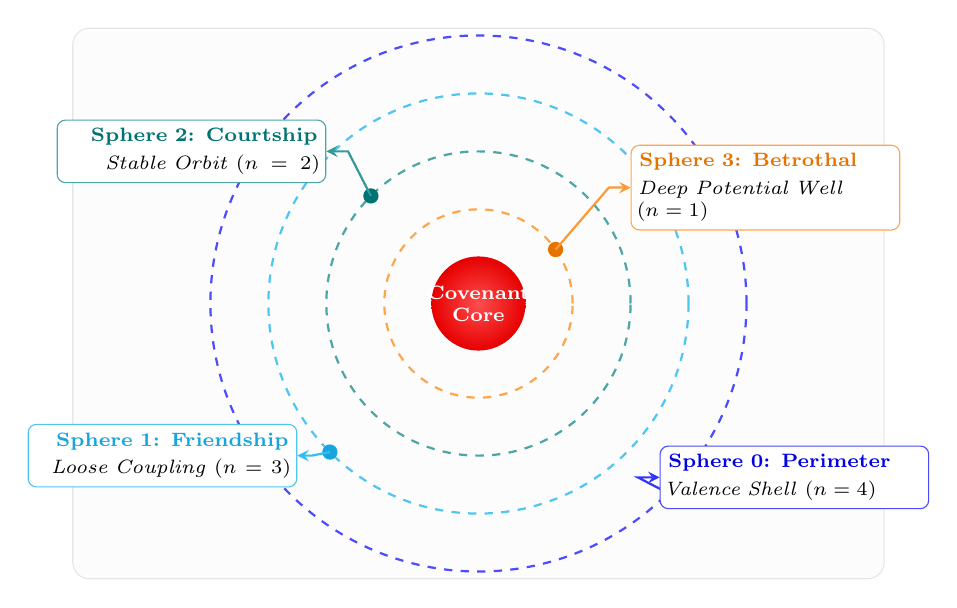
\begin{tikzpicture}[scale=0.92, >=stealth]
  \draw[gray!20, fill=gray!2, rounded corners=6pt] (-5.6, -3.8) rectangle (5.6, 3.8);

  % Core Nucleus
  \shade[inner color=red!70, outer color=red!90!black] (0,0) circle (0.65cm);
  \node[font=\bfseries\scriptsize, white, align=center] at (0,0) {Covenant\\Core};

  % Concentric Orbits
  \draw[thick, orange!70, dashed] (0,0) circle (1.3cm);
  \draw[thick, teal!70, dashed] (0,0) circle (2.1cm);
  \draw[thick, cyan!70, dashed] (0,0) circle (2.9cm);
  \draw[thick, blue!70, dashed] (0,0) circle (3.7cm);

  % Particles
  \fill[orange!90!black] (35:1.3cm) circle (3pt);
  \fill[teal!90!black] (135:2.1cm) circle (3pt);
  \fill[cyan!90!black] (225:2.9cm) circle (3pt);
  \fill[blue!90!black] (315:3.7cm) circle (3pt);

  % Callouts
  \draw[thick, orange!80, ->] (35:1.3cm) to (1.8, 1.6) to (2.1, 1.6);
  \node[anchor=west, font=\scriptsize, fill=white, draw=orange!70, rounded corners=3pt, inner sep=3pt, text width=3.2cm, align=left] at (2.1, 1.6) {
    \textbf{\textcolor{orange!90!black}{Sphere 3: Betrothal}}\\[2pt]
    \textit{Deep Potential Well} ($n=1$)
  };

  \draw[thick, teal!80, ->] (135:2.1cm) to (-1.8, 2.1) to (-2.1, 2.1);
  \node[anchor=east, font=\scriptsize, fill=white, draw=teal!70, rounded corners=3pt, inner sep=3pt, text width=3.2cm, align=right] at (-2.1, 2.1) {
    \textbf{\textcolor{teal!90!black}{Sphere 2: Courtship}}\\[2pt]
    \textit{Stable Orbit} ($n=2$)
  };

  \draw[thick, cyan!80, ->] (225:2.9cm) to (-2.3, -2.1) to (-2.5, -2.1);
  \node[anchor=east, font=\scriptsize, fill=white, draw=cyan!70, rounded corners=3pt, inner sep=3pt, text width=3.2cm, align=right] at (-2.5, -2.1) {
    \textbf{\textcolor{cyan!90!black}{Sphere 1: Friendship}}\\[2pt]
    \textit{Loose Coupling} ($n=3$)
  };

  \draw[thick, blue!80, ->] (315:3.7cm) to (2.2, -2.4) to (2.5, -2.4);
  \node[anchor=west, font=\scriptsize, fill=white, draw=blue!70, rounded corners=3pt, inner sep=3pt, text width=3.2cm, align=left] at (2.5, -2.4) {
    \textbf{\textcolor{blue!90!black}{Sphere 0: Perimeter}}\\[2pt]
    \textit{Valence Shell} ($n=4$)
  };
\end{tikzpicture}
\caption{\textbf{Atomic Orbital Model of Courtship Physics.} Moving inward toward the covenant core requires verified binding energy and deliberate state transitions.}
\label{fig:atomicshell}
\end{figure}

\chapter{The Two Springs of Commitment: Stanley and Markman}

\section{Dedication versus Constraint}
``Let us examine how couples get trapped,'' Feynman said, drawing two mechanical springs side by side on the slate.

``Social scientists Scott Stanley and Howard Markman discovered that commitment consists of two independent mechanical forces,'' Feynman explained:
\begin{enumerate}
    \item \textbf{Dedication Commitment}: The internal drive to build a shared future, prioritize partner welfare, and cultivate an identity as `we.'
    \item \textbf{Constraint Commitment}: The external friction making exit costly, such as shared leases, financial debt, social disapproval, and co-parenting entanglements.
\end{enumerate}

``Imagine a heavy freight car on a railroad track,'' Feynman said. ``If you push the car into motion without brakes, friction and momentum take over. Stanley calls this `sliding versus deciding.' Secular dating encourages couples to slide: they start dating casually, slide into sexual intimacy, slide into signing an apartment lease to save rent money, and suddenly find massive constraints holding them together before they ever tested each other's dedication.''

``They accumulate constraints before verifying character,'' Daniel said.

``Exactly!'' Feynman said. ``The couple wakes up three years later. They fight constantly. They disagree on God, children, and money. Yet they feel trapped because breaking the apartment lease costs money and their families expect a wedding. They marry out of pure inertia. Five years later, under real stress, the fragile structure explodes.''

``How does Christian courtship invert that process?''

``By decoupling dedication from constraint during vetting,'' Feynman replied. ``In Christian courtship, you deliberately hold constraints low while testing dedication under observation. You maintain separate households. You invite pastoral scrutiny. You measure character across months of ordinary life. You make conscious, sober decisions at every threshold.''

\begin{figure}[H]
\centering
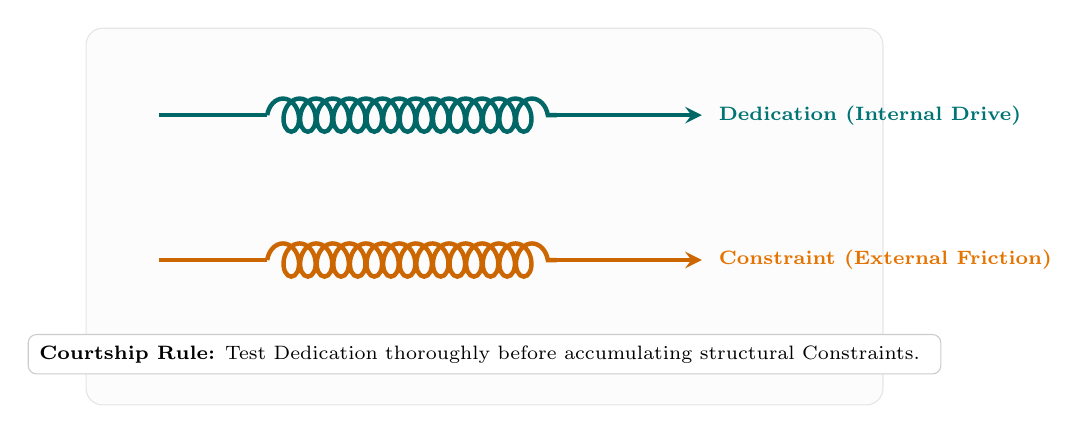
\begin{tikzpicture}[scale=0.92, >=stealth]
  \draw[gray!20, fill=gray!2, rounded corners=6pt] (-1.0, -1.0) rectangle (10.0, 4.2);

  % Dedication Spring
  \draw[ultra thick, teal!80!black] (0, 3.0) to (1.5, 3.0);
  \draw[ultra thick, teal!80!black, decorate, decoration={coil, aspect=0.7, segment length=6pt, amplitude=6pt}] (1.5, 3.0) to (5.5, 3.0);
  \draw[ultra thick, teal!80!black, ->] (5.5, 3.0) to (7.5, 3.0);
  \node[anchor=west, font=\scriptsize\bfseries, text=teal!90!black] at (7.6, 3.0) {Dedication (Internal Drive)};

  % Constraint Spring
  \draw[ultra thick, orange!80!black] (0, 1.0) to (1.5, 1.0);
  \draw[ultra thick, orange!80!black, decorate, decoration={coil, aspect=0.7, segment length=6pt, amplitude=6pt}] (1.5, 1.0) to (5.5, 1.0);
  \draw[ultra thick, orange!80!black, ->] (5.5, 1.0) to (7.5, 1.0);
  \node[anchor=west, font=\scriptsize\bfseries, text=orange!90!black] at (7.6, 1.0) {Constraint (External Friction)};

  \node[font=\scriptsize, align=center, fill=white, draw=gray!40, rounded corners=3pt, inner sep=4pt] at (4.5, -0.3) {
    \textbf{Courtship Rule:} Test Dedication thoroughly before accumulating structural Constraints.
  };
\end{tikzpicture}
\caption{\textbf{The Two-Spring Commitment Model.} Internal dedication must lead relational growth, preventing constraint-driven inertia.}
\label{fig:twosprings}
\end{figure}

\chapter{Thermal Noise, Differentiation of Self, and the Three Traditions}

\section{Murray Bowen and Emotional Fusion}
Feynman drew a temperature scale on the blackboard.

``Let us talk about thermal stability,'' Feynman said. ``Murray Bowen founded family systems theory around a central concept: Differentiation of Self. In thermodynamics, high thermal noise causes molecules to vibrate chaotically, losing their crystalline structure. Low-differentiation individuals are emotionally overheated: they fuse with other people. When their partner is anxious, they panic. When their partner is angry, they become defensive. They oscillate between enmeshment and emotional cutoff.''

``I felt that in my first marriage,'' Daniel admitted. ``When she panicked about money, I took on false guilt. I tried to control her moods to calm my own anxiety.''

``A classic failure of differentiation,'' Feynman said. ``A differentiated Christian maintains a clear `I-position' grounded in Christ while sustaining deep connection with others. You stay calm when your partner is distressed. You state your convictions with quiet firmness. You offer compassion without absorption.''

\section{The Three Great Traditions}
Feynman wrote three names across the board: Wittenberg, Rome, and Constantinople.

``To build an unbreakable courtship, you synthesize three ancient reservoirs of wisdom,'' Feynman explained:
\begin{enumerate}
    \item \textbf{The Protestant Pillar} (Martin Luther and John Calvin): Marriage is a holy creation ordinance and public covenant. Luther emphasized mutual affection, daily companionship, and protection against sin. Calvin insisted on community accountability: parental counsel, church consistory oversight, and civil transparency. You date inside the church family, not in secret corners.
    \item \textbf{The Catholic Pillar} (Thomas Aquinas and Karol Wojtyla): Marriage is a sacred reality (\textit{matrimonium}). Aquinas taught that the efficient cause of marriage is mutual consent in words of the present tense (\textit{per verba de praesenti}), which must be clearly separated from forward promises (\textit{sponsalia de futuro}). Wojtyla formulated the personalistic norm: a human person is a subject of dignity, never an object of consumption or physical utility.
    \item \textbf{The Eastern Orthodox Pillar} (St.~John Chrysostom and the Crowning): Marriage is an icon of the Kingdom of God. In the Orthodox mystery of crowning (\textit{Stephana}), the crowns placed upon the couple represent the crowns of martyrdom: dying to selfish ego and pride. The home becomes a little church (\textit{ecclesiola}). The Orthodox tradition cultivates watchfulness (\textit{nepsis}) and sober discernment (\textit{diakrisis}).
\end{enumerate}

\chapter{The Core Guardrail: Why You Can't Touch the Stove}

\section{The Physics of Premarital Chastity}
Feynman leaned over his desk, his eyes sharp. ``Now we come to the hardest law of the entire course. The universal rule that every young person wants to negotiate: no doing the deal before marriage.''

Daniel shifted in his chair. ``It is the hardest rule in the world, Professor. When you care deeply for someone, every instinct pulls toward physical closeness.''

``Of course it does!'' Feynman barked, grinning. ``Nature designed the physical mechanism with immense power. But let us look at the physics. Why does God command absolute premarital chastity? Is He trying to spoil your weekend? Or is He protecting the machinery of your soul?''

Feynman drew a chemical synapse on the board.

``When two human beings engage in sexual union,'' Feynman said, ``the brain floods with oxytocin, dopamine, and vasopressin. These neurochemicals act as superglue. They generate intense emotional attachment and cloud critical judgment. If you engage in physical intimacy before marriage, your brain releases bonding chemicals that trick you into feeling safe with someone who may be a liar, an abuser, or an unfaithful partner.''

``It creates false intimacy,'' Daniel said.

``It short-circuits your evaluation instruments!'' Feynman said loudly. ``Imagine an airplane pilot flying through thick clouds. He needs to read his altimeter and airspeed indicator with total clarity. If he pours sticky syrup all over the cockpit dials, he cannot tell whether he is flying level or diving straight into a mountain. Premarital sex pours syrup over your cognitive instruments. You mistake physical euphoria for spiritual compatibility.''

Feynman tapped the board. ``First Thessalonians four, three through five commands: abstain from sexual immorality; control your own vessel in holiness and honor. First Corinthians six, eighteen commands: flee fornication. The body is a temple of the Holy Spirit. Consummation belongs exclusively inside the lifelong covenant of marriage (Sphere 4). Keeping your hands off each other during courtship is non-negotiable safety physics. It preserves the sober mind you need to evaluate whether you should pledge your life to this person.''

\chapter{Deception, Defection, and the Quarantine Valve}

\section{Realism Regarding Fallen Humanity}
``Let us dispense with sentimental fairy tales,'' Feynman said, pacing the room. ``Human beings are fallen creatures. Spouses lie. Boyfriends cheat. Fiances hide thirty thousand dollars in credit card debt. Believers backslide into pornography or alcoholism. If your courtship system assumes your partner is an angel, your system will crash.''

``What is the game-theoretic defense?'' Daniel asked.

``Longitudinal verification,'' Feynman replied. ``You do not accept verbal claims at face value. Talk is cheap. You observe behavior across time under pressure. You watch how they treat a rude waiter. You observe how they react when their plans get canceled. You verify their bank statements and debt obligations before betrothal.''

\section{The Quarantine and Revocation Circuit Breakers}
Feynman drew a state machine with a safety valve:
\begin{enumerate}
    \item \textbf{Quarantine Valve}: If an unverified inconsistency or moral concern surfaces during courtship, all escalation halts instantly. Interaction drops to public settings under pastoral guidance for ninety days.
    \item \textbf{Immediate Revocation}: If active deceit, physical boundary violation, or infidelity occurs, the courtship terminates instantly. The state machine executes a hard reset back to Sphere 0.
\end{enumerate}

``What about forgiveness?'' Daniel asked. ``Jesus commands forgiving seventy times seven.''

``Listen carefully,'' Feynman said, pointing his finger. ``Forgiveness is unilateral; trust is earned. You forgive the person in your heart immediately so that bitterness does not rot your spirit. You surrender all desire for revenge to God. But you do not marry them! Forgiving a thief does not mean handing him the keys to the bank vault. Forgiveness clears the past; trust requires verified future performance.''

\chapter{The Inverted Engine: Learning from the Wreckage}

\section{The Tragedy of Daniel's Past Marriage}
Feynman sat down next to Daniel, speaking with quiet gravity. ``Daniel, tell me about your former wife.''

Daniel looked down at his hands, calloused from the machine shop lathe. ``We met in college. We were young. We felt overwhelming chemistry. We never talked about theology, money, or the cross. We slid into marriage because everyone expected it. When my father suffered his stroke and the machine shop almost went under, the pressure mounted. Maddie was born with health challenges. My former wife hated the sacrifice. She resented the shop, resented my prayers, and eventually walked away with an associate from the city. She wanted a lifestyle, not a covenant. The elders tried to intervene, but she refused all reconciliation. She declared she had no faith in Christ.''

``A catastrophic failure of the foundation,'' Feynman said gently. ``Scripture recognizes this tragedy in First Corinthians seven, fifteen: if the unbelieving partner departs, the brother or sister is not bound. God calls us to peace. Yet divorce is always a tearing of one flesh. It leaves deep scars.''

``It felt like total failure,'' Daniel whispered.

``It was a failure of structure,'' Feynman said. ``And that failure is your greatest teacher. In aviation, every air safety rule is written in the wreckage of past crashes. Engineers study the twisted metal to discover why the wing tore off. Your first marriage crashed because it was built on sliding, unvetted character, and lack of spiritual alignment. That painful history is your inverted engine: it teaches you precisely what you must never compromise on with Nora.''

``With Nora, everything is different,'' Daniel said softly. ``We started as friends. She sat with me on the porch. She challenged my sloppy boundaries. She knows about Maddie and loves her. We pray together.''

``Then honor the physics,'' Feynman said, clapping him on the shoulder. ``Move through the concentric spheres with holy patience: from faithful friendship to deliberate courtship, testing character at every gate, guarding physical purity with unbending resolve, until the day you stand before God and receive the crown of covenant marriage.''

\chapter{Worked Socratic Dialogues and In-Class Case Studies}

\section{Case Study 1: The Concealed Debt Dilemma}
Daniel presents the case of suitor Thomas and candidate Sarah. Two months into deliberate courtship (Sphere 2), Thomas discovers that Sarah has concealed fifteen thousand dollars in delinquent consumer credit card debt. When confronted, Sarah cries and claims she was ashamed to tell him.

\begin{blackboard}
\textbf{In-Class Dialogue Analysis:}\\
\textbf{Feynman:} ``Apply the framework, Daniel. What does the state machine do?''\\
\textbf{Daniel:} ``This is an active concealment of material facts. It violates the integrity metric.''\\
\textbf{Feynman:} ``Does Thomas immediately dump her?''\\
\textbf{Daniel:} ``He activates the Quarantine Valve. All wedding or betrothal talk halts. They consult pastoral counsel. Sarah must demonstrate transparent financial budgeting and active debt repayment across six months of verified accounting. If she becomes defensive or blames others, Thomas executes immediate revocation.''\\
\textbf{Feynman:} ``Correct! Mercy offers a path to restitution; wisdom withholds the keys until the debt is cleared.''
\end{blackboard}

\chapter{End-of-Chapter Homework Assignments and Thought Experiments}

\section{Thought Experiment 1: The Pressure Test}
You are in deliberate courtship (Sphere 2). Your courtship partner proposes a weekend getaway together in a mountain cabin, promising to sleep in separate beds to save money and enjoy nature. 
\begin{enumerate}
    \item Identify the structural hazard of this proposal using commitment theory.
    \item Formulate the exact verbal response enforcing the physical boundary invariant.
\end{enumerate}

\begin{blackboard}
\textbf{Solution Outline:}
\begin{enumerate}
    \item \textit{Structural Hazard}: Isolated domestic cohabitation creates extreme sexual temptation, violates the public witness of the church, and induces premature constraint inertia.
    \item \textit{Scripted Response}: ``I value our future and honor God's boundary. We will not share an isolated cabin. We will plan day trips with friends or stay in separate locations with family.''
\end{enumerate}
\end{blackboard}

\chapter{Examinations and Solutions}

\section{Midterm Examination}

\paragraph{Question 1: Mathematical Foundations}
Define the mathematical loss function of courtship defection versus cooperation. Explain why secular dating markets produce high defection rates, and demonstrate how ecclesiastical accountability converts courtship into an assurance coordination game.

\begin{blackboard}
\textbf{Midterm Solution 1:}
In unconstrained dating markets, the temptation payoff $T$ exceeds mutual cooperation $R$, creating a prisoner's dilemma where defection dominates. By introducing ecclesiastical and community penalties $K_{\text{church}}$ where $K_{\text{church}} > T - R$, the payoff of defection drops to $T - K_{\text{church}}$, rendering mutual cooperation ($C, C$) the unique stable equilibrium.
\end{blackboard}

\section{Comprehensive Final Examination}

\paragraph{Scenario: The Second Courtship Under Historical Scrutiny}
A believer who experienced a biblical divorce under First Corinthians seven, fifteen seeks to enter courtship with a mature Christian woman. Outline the comprehensive four-phase verification process required before solemn betrothal, incorporating Protestant pastoral counsel, Catholic personalistic dignity, and Orthodox ascetical watchfulness.

\begin{blackboard}
\textbf{Final Exam Solution:}
\begin{enumerate}
    \item \textbf{Phase 1}: Complete pastoral audit of the prior divorce, confirming unpreventable abandonment by an unbelieving spouse, full resolution of parental obligations, and freedom from lingering bitterness.
    \item \textbf{Phase 2}: Six months of community observation within local church life, verifying emotional differentiation and stable paternal care.
    \item \textbf{Phase 3}: Formal deliberate courtship establishing mutual doctrinal unity, financial transparency, and strict physical chastity.
    \item \textbf{Phase 4}: Final consistory clearance and betrothal pledge under solemn witness, moving toward holy matrimony as an enduring covenant.
\end{enumerate}
\end{blackboard}

\end{document}
